\documentclass[12pt]{article}%
\usepackage[paper=portrait,pagesize]{typearea}
\usepackage{amssymb}
\usepackage{amsfonts}
\usepackage{amsmath}
\usepackage{hyperref}
\usepackage{lscape}
\usepackage{comment}
\usepackage[flushleft]{threeparttable}
\usepackage{float}
\usepackage[nohead]{geometry}
\usepackage[singlespacing]{setspace}
\usepackage[paper=portrait,pagesize]{typearea}
\usepackage{amssymb}
\usepackage{amsfonts}
\usepackage{multicol}
\usepackage{amsmath}
\usepackage{hyperref}
\usepackage[nameinlink,noabbrev]{cleveref}
\usepackage{lscape}
\usepackage{float}
\usepackage[nohead]{geometry}
\usepackage[singlespacing]{setspace}
\usepackage[bottom]{footmisc}
\usepackage{indentfirst}
\usepackage{endnotes}
\usepackage{graphicx}%
\usepackage{afterpage}
\usepackage{subfig}
\usepackage{rotating}
\newcommand\tab[1][1cm]{\hspace*{#1}}
\DeclareMathOperator*{\Max}{Max}
\newcommand\numberthis{\addtocounter{equation}{1}\tag{\theequation}}
\def\dotfill#1{\cleaders\hbox to #1{.}\hfill}
\newcommand\dotline[2][.5em]{\leavevmode\hbox to #2{\dotfill{#1}\hfil}}
%\usepackage[backend=biber,style=alphabetic,sorting=ynt]{biblatex}
%\addbibresource{bibliocopulas.bib}
\usepackage[round,sort,comma,authoryear]{natbib}
\setcounter{MaxMatrixCols}{30}
\newtheorem{theorem}{Theorem}
\newtheorem{acknowledgement}{Acknowledgement}
\newtheorem{algorithm}[theorem]{Algorithm}
\newtheorem{axiom}[theorem]{Axiom}
\newtheorem{case}[theorem]{Case}
\newtheorem{claim}[theorem]{Claim}
\newtheorem{conclusion}[theorem]{Conclusion}
\newtheorem{condition}[theorem]{Condition}
\newtheorem{conjecture}[theorem]{Conjecture}
\newtheorem{corollary}[theorem]{Corollary}
\newtheorem{criterion}[theorem]{Criterion}
\newtheorem{definition}[theorem]{Definition}
\newtheorem{example}[theorem]{Example}
\newtheorem{exercise}[theorem]{Exercise}
\newtheorem{lemma}[theorem]{Lemma}
\newtheorem{notation}[theorem]{Notation}
\newtheorem{problem}[theorem]{Problem}
\newtheorem{proposition}{Proposition}
\newtheorem{remark}[theorem]{Remark}
\newtheorem{solution}[theorem]{Solution}
\newtheorem{summary}[theorem]{Summary}
\newenvironment{proof}[1][Proof]{\noindent\textbf{#1.} }{\ \rule{0.5em}{0.5em}}
\newcommand{\pd}[2]{\frac{\partial#1}{\partial#2}}
\makeatletter
\def\@biblabel#1{\hspace*{-\labelsep}}
\makeatother
\geometry{left=1in,right=1in,top=1.00in,bottom=1.0in}
%\renewcommand*\abstractname{Summary}

\begin{document}

\title{Fall 2019 - ECON 634 - Advance Macroeconomics - Problem Set 2}
\author{Elisa Taveras Pena\footnote{E-mail address: \href{mailto:etavera2@binghamton.edu}{etavera2@binghamton.edu}  }\\
Binghamton University}
\maketitle

\sloppy%avoids the breakage of words at the end of lines, by adjusting spaces between words inside the lines

\onehalfspacing

\begin{enumerate}
	\item 
	
	Since the Resource constraint (Social Planner Problem) is $c_t=A_tk_{t}^\alpha+(1-\delta)k_{t}-k_{t+1}$ we can write the budget constraint  in recursive form as  $c=Ak^\alpha+(1-\delta)k-k'$ 
	
	\tab \textbf{ $\bullet$ State variable}: $k,A$ 
	
	\tab \textbf{ $\bullet$ Control variable}: $k'$
	
	
	
	Therefore, the Bellman equation:
	
	\begin{align*}
	&V(k,A)=\Max_{k'} \left\lbrace \frac{\left( Ak^\alpha+(1-\delta)k-k'\right) ^{1-\sigma}}{1-\sigma}+ \beta \sum_{A' \in A} \Pi(A'|A)V(k',A')\right\rbrace 
	& \notag \\
	&\text{subject to} \notag \\
	& \tab c \in [0,f(k)] \numberthis\\
	& \tab k' \in [0,f(k)] \ \numberthis\\
	\end{align*} 
	
	\item Using the VFI, the Graphs are like follows:
	
	\begin{center}
		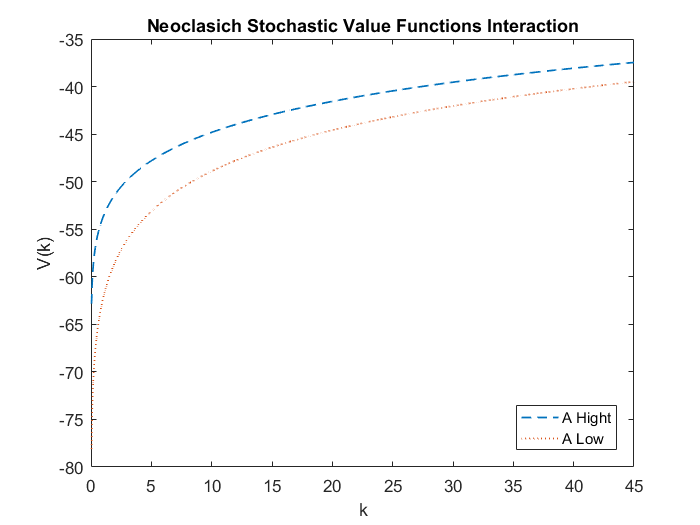
\includegraphics[width=1\linewidth]{VF}
	\end{center}
	
	
	As we can see, both are increasing and concave functions. 
	
	\item  The Policy function over $k$ looks as follows:
	
	\begin{center}
		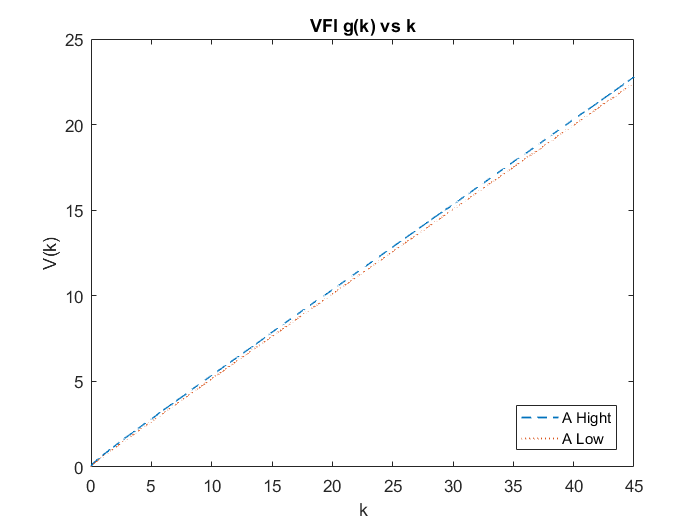
\includegraphics[width=1\linewidth]{g_k}
	\end{center}

This relationship is decreasing in $k$ but increasing in $A$.
	
	Assuming that by saving, it means what is left from production after consumption: $s=k^{\prime}-(1-\delta)k$, the Saving over $k$ looks as follows:
	
	\begin{center}
		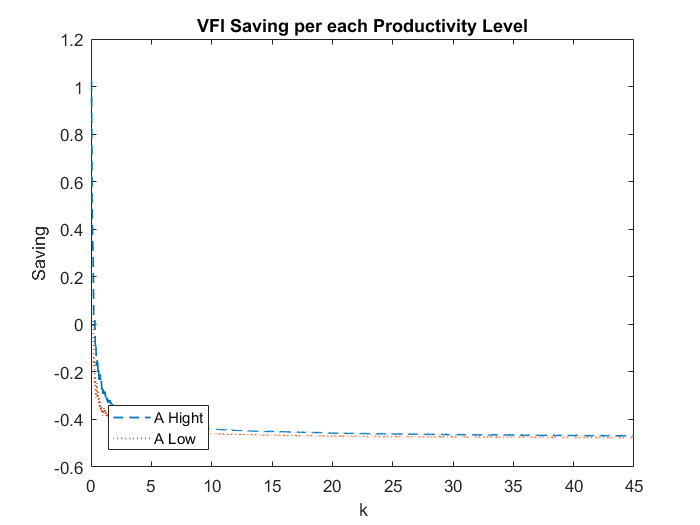
\includegraphics[width=1\linewidth]{saving}
	\end{center}
	
	where this relationship is decreasing in $k$ and increasing in $A$. This make sense because 

	
	\item For this, I will use the code for the part (5), since it seems more reasonable results.  Using the results, I get a $sd(y)=0.1755$, whci does not match the results from the data. Doing the markov change process to find stationary probabilities:
	
		\[
	\begin{pmatrix}\bar{\pi}_{h} & \bar{\pi}_{l}\end{pmatrix}=\begin{pmatrix}\bar{\pi}_{h} & \bar{\pi}_{l}\end{pmatrix}P
	\]
	
	This means
	
	\[
	\begin{pmatrix}\bar{\pi}_{h} & \bar{\pi}_{l}\end{pmatrix}=\begin{pmatrix}\bar{\pi}_{h} & \bar{\pi}_{l}\end{pmatrix}\left[\begin{array}{cc}
	0.977 & 0.023\\
	0.074 & 0.926
	\end{array}\right],
	\]
	
			\[
	\begin{pmatrix}\bar{\pi}_{h} & \bar{\pi}_{l}\end{pmatrix}=\begin{pmatrix} 0.977\bar{\pi}_{h}+ 0.074\bar{\pi}_{l} & 	0.023\bar{\pi}_{h}+0.926\bar{\pi}_{l}\end{pmatrix},
	\]
	
		Therefore,
	
	\begin{align*}
	&\bar{\pi}_{h}=  3.22 \bar{\pi}_{l}  \numberthis \\
	&\bar{\pi}_{l}=  0.31 \bar{\pi}_{h} \numberthis \\	
	\end{align*}
	
		Since $\bar{\pi}_{h}+\bar{\pi}_{l}=1$
	
	\begin{align*}
	&4.22\bar{\pi}_{l}= 1 \numberthis \\
	&\bar{\pi}_{l}= 0.24  \numberthis \\
	&\bar{\pi}_{h}=  0.76   \numberthis \\	
	\end{align*}
	
	 Therefore, I will try first, $A_h=1.05$, which implies sung the Long-run probabilities $A_l=\frac{1-\bar{\pi_h}A_h}{\bar{\pi_l}}= 0.839$. With this results, the standard deviation is $sd(y)=0.1445$, which means I need to keep trying for a smaller value of $A_h$. Using $A_h=1.00005$, $A_l= 0.99984$, then 
	 
	 
	 Ideally, I should do a while loop and try for a low tolerance between my simulated standard deviation and the actual standard deviation. Because the code \textbf{VFIP5} is so slow, I decide against it and just try randomly picking a number.	 	 
	 
	
	\item See Code \textbf{VFIP5}. Using two loops over all $K$ is quite slow and does spend a long time to find a solution. 
	
	The time on the previous program \textbf{Elapsed time is 0.326278 seconds.}
	For the second one, limiting to the  \textbf{Elapsed time is 1049.453223 seconds.} Therefore, time is significantly higher for this one. 
	
	Since, to me, this second version is correct, but I get differents results, I will add the graphs for this. The results for the VFI is: 
	
	\begin{center}
		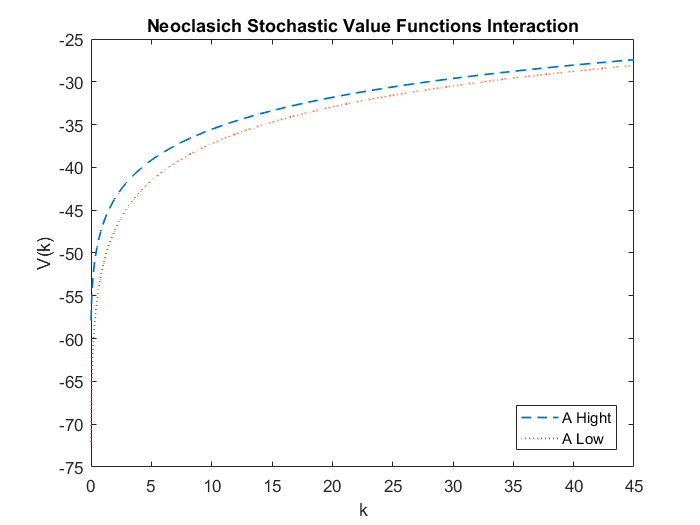
\includegraphics[width=1\linewidth]{VFP5}
	\end{center}
	
	\begin{center}
		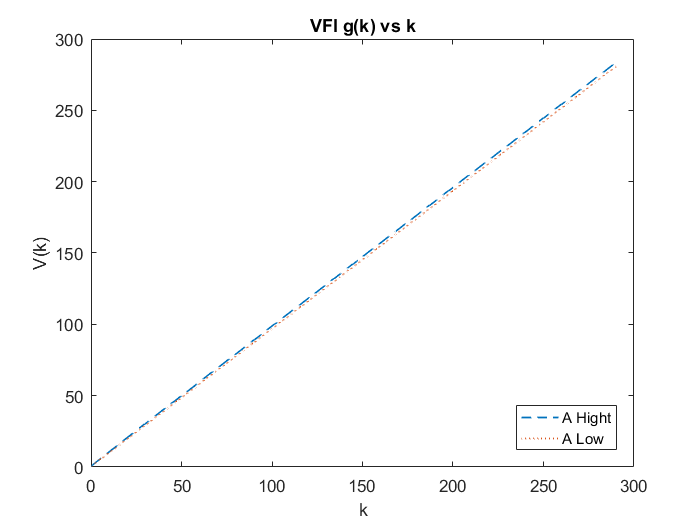
\includegraphics[width=0.7\linewidth]{g_kP5}
	\end{center}

	\begin{center}
		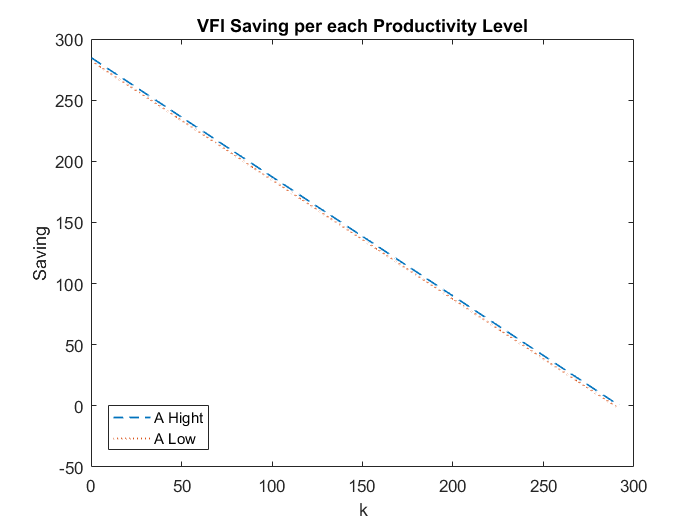
\includegraphics[width=0.7\linewidth]{savingP5}
	\end{center}
	
	
	
\end{enumerate}

\strut

\onehalfspacing

\end{document}
